%\documentclass[preprint]{sigplanconf}
%\documentclass[preprint]{llncs}
\documentclass[a4paper,UKenglish]{lipics}

\usepackage{microtype}%if unwanted, comment out or use option "draft"
\usepackage[table,xcdraw]{xcolor}
\usepackage{color}
\usepackage{amsmath}
\usepackage{stmaryrd}
\usepackage{graphicx}
\usepackage{amssymb}
\usepackage{fancyvrb}
\usepackage{url}
\usepackage{pstricks,pst-node,pst-tree}
\usepackage{theorem}
%% \usepackage{mathpartir}
\usepackage{bbm}
\usepackage{pgf}
\usepackage{multirow}

\usepackage{listings}
\usepackage{verbatim}
\usepackage{graphicx}
\usepackage{wrapfig}

\usepackage[T1]{fontenc}
\usepackage[scaled=0.85]{beramono}
\usepackage{mathpartir}

% "define" code highlights for Java and Scala
\lstdefinelanguage{JavaScala}{
  morekeywords={public,int,interface,implements,default,
    abstract,case,catch,class,def,static,%
    do,else,extends,false,final,finally,%
    for,if,implicit,import,match,mixin,%
    new,null,object,override,package,%
    private,protected,requires,return,sealed,%
    super,this,throw,trait,true,try,%
    type,var,while,yield,with,val},
  otherkeywords={=>,<-,<\%,<:,>:,\#,@},
  sensitive=true,
  morecomment=[l]{//},
  morecomment=[n]{/*}{*/},
  morestring=[b]",
  morestring=[b]',
  morestring=[b]"""
}

\lstset{ %
language=JavaScala,                % choose the language of the code
columns=flexible,
lineskip=-1pt,
basicstyle=\ttfamily\small,       % the size of the fonts that are used for the code
numbers=none,                   % where to put the line-numbers
numberstyle=\ttfamily\tiny,      % the size of the fonts that are used for the line-numbers
stepnumber=1,                   % the step between two line-numbers. If it's 1 each line will be numbered
numbersep=5pt,                  % how far the line-numbers are from the code
backgroundcolor=\color{white},  % choose the background color. You must add \usepackage{color}
showspaces=false,               % show spaces adding particular underscores
showstringspaces=false,         % underline spaces within strings
showtabs=false,                 % show tabs within strings adding particular underscores
morekeywords={var},
%  frame=single,                   % adds a frame around the code
tabsize=2,                  % sets default tabsize to 2 spaces
captionpos=none,                   % sets the caption-position to bottom
breaklines=true,                % sets automatic line breaking
breakatwhitespace=false,        % sets if automatic breaks should only happen at whitespace
title=\lstname,                 % show the filename of files included with \lstinputlisting; also try caption instead of title
escapeinside={(**}{**)},          % if you want to add a comment within your code
keywordstyle=\ttfamily\bfseries,
% commentstyle=\color{Gray},
% stringstyle=\color{Green}
}


%%\usepackage{natbib}
%%\bibpunct();A{},
%%\let\cite=\citep

%include lhs2TeX.fmt
%include lhs2TeX.sty
%include forall.fmt

%\pagestyle{plain}

%{\theorembodyfont{\sffamily} \newtheorem{theorem}{Theorem}}
%{\theorembodyfont{\sffamily} \newtheorem{lemma}{Lemma}}
%\newtheorem{theorem}{Theorem}
%\newtheorem{lemma}{Lemma}
%\newenvironment{proof}{\textbf{Proof:\hspace{4mm}}}{$\Box$}
\newcommand{\authornote}[3]{{\color{#2} {\sc #1}: #3}}
\newcommand\bruno[1]{\authornote{bruno}{red}{#1}}
\newcommand\yanlin[1]{\authornote{yanlin}{purple}{#1}}
%\newcommand{\hl}[1]{\textcolor{red}{#1}}
\newcommand\huang[1]{\authornote{huang}{blue}{#1}}
\newcommand\haoyuan[1]{\authornote{haoyuan}{cyan}{#1}}

\newcommand\sem[1]{\llbracket #1 \rrbracket_r}
\newcommand\sems[1]{\llbracket #1 \rrbracket_s}
\newcommand\tsem[1]{\llbracket #1 \rrbracket}
\newcommand{\rbm}[1]{\raisebox{-2.0ex}[0.5ex]{#1}}
\newcommand\nat[0]{\mathbb{N}}
\newcommand\unit[0]{\mathbbm{1}}

\newcommand\mixin{\textbf{@Mixin} }
\usepackage{xspace}

% Author macros::begin %%%%%%%%%%%%%%%%%%%%%%%%%%%%%%%%%%%%%%%%%%%%%%%%
\title{Type-Safe Modular Parsing}
\titlerunning{Type-Safe Modular Parsing}

\author[1]{John Q. Open}
\author[2]{Joan R. Access}
\affil[1]{Dummy University Computing Laboratory\\
  Address, Country\\
  \texttt{open@dummyuni.org}}
\affil[2]{Department of Informatics, Dummy College\\
  Address, Country\\
  \texttt{access@dummycollege.org}}
\authorrunning{J.\,Q. Open and J.\,R. Access}
% mandatory. First: Use abbreviated first/middle names. Second (only in severe
% cases): Use first author plus 'et. al.'

\Copyright{John Q. Open and Joan R. Access}
% mandatory, please use full first names. LIPIcs license is "CC-BY";
% http://creativecommons.org/licenses/by/3.0/

\subjclass{Dummy classification -- please refer to
  \url{http://www.acm.org/about/class/ccs98-html}}
% mandatory: Please choose ACM 1998 classifications from
% http://www.acm.org/about/class/ccs98-html . E.g., cite as "F.1.1 Models of
% Computation".
\keywords{Dummy keyword -- please provide 1--5 keywords}% mandatory: Please provide 1-5 keywords
% Author macros::end %%%%%%%%%%%%%%%%%%%%%%%%%%%%%%%%%%%%%%%%%%%%%%%%%

%Editor-only macros:: begin (do not touch as author)%%%%%%%%%%%%%%%%%%%%%%%%%%%%%%%%%%
\serieslogo{}%please provide filename (without suffix)
\volumeinfo%(easychair interface)
  {Billy Editor and Bill Editors}% editors
  {2}% number of editors: 1, 2, ....
  {Conference title on which this volume is based on}% event
  {1}% volume
  {1}% issue
  {1}% starting page number
\EventShortName{}
\DOI{10.4230/LIPIcs.xxx.yyy.p}% to be completed by the volume editor
% Editor-only macros::end %%%%%%%%%%%%%%%%%%%%%%%%%%%%%%%%%%%%%%%%%%%%%%%

%%%%%%%%%%%%%%%%%%%%%%%%%%%%%%%%%%%%%%%%%%%%%%%%%%%%%%%%%%%%%%%%%%%%%%%%%%%%%%%%
\begin{document}
\maketitle

\begin{abstract}

Text.

\end{abstract}

%if False

%\category{D.3.2}{Programming Languages}
%                {Language Classifications}
%                [Functional Languages]
%\category{F.3.3}{Logics and Meanings of Programs}
%                {Studies of Program Constructs}
%                []

%\terms
%Languages
%
%\keywords
%Mixins, explicit effects, monads, aspect-oriented programming, parametricity,
%interference

%endif

%===============================================================================

\section{Introduction}\label{sec:introduction}
 
The quest for improved modularity, variability and extensibility of
programs has been going on since the early days of Software
Engineering~\cite{McIlroy68}. Modern Programming Languages (PLs) enable a certain
degree of modularity, but they have limitations as illustrated by
well-known problems such as the Expression Problem~\cite{wadler1998expression}. The
Expression Problem refers to the difficulty of writing data
abstractions that can be easily extended with both new operations and
new data variants. Traditionally the kinds of data abstraction found
in functional languages can be extended with new operations, but
adding new data variants is difficult. The traditional object-oriented
approach to data abstraction facilitates adding new data variants
(classes), while adding new operations is more difficult.

\begin{comment}
A reason why a solution to the Expression Problem is important in
practice is that it is necessary for the development of
\emph{Software-Product Lines} (SPLs)~\cite{}. A software-product line
is a reusable set of components, which can be combined in multiple ways
to obtain different programs. Programming languages offer a concrete
example for SPLs. A SPL for programming languages would allow us to
model various typical operations of programming languages (such as
evaluation, compilation, or parsing) for various different language
constructs (such as binding, arithmetic, conditional or loops)
independently and separately. For example, evaluation components could be defined
independently for binding and arithmetic constructs. If the language
to be implemented is the pure lambda calculus, only evaluation of
binding constructs is necessary. However, more realistic programming
languages will include arithmetic constructs, and will require 
evaluation for such constructs as well. In this case 
both the component for evaluation of binders and arithmetic 
expressions can be combined to implement the desired functionality.
\end{comment}

\begin{comment}
Most programming languages share alot of features in
common. 

For example, most languages have language constructs for:
binding (such as variables, functions, and function applications);
basic arithmetic operations; basic logic and conditional operations;
loops; as well as various other features. For each language construct,
various operations (such as evaluation, compilation, or parsing) need
to be implemented. It is reasonable to wonder whether we can simply
implement those features independently of a particular implementation
of a programming language. Evaluation could be defined independently 
for binding and arithmetic constructs. If the language to be
implemented is the pure lambda calculus, only evaluation of binding 
constructs is necessary. Thus only the component that implements 
evaluation for binding needs to be used in such an implementation.
However, more realistic programming languages 
will include arithmetic constructs, and will require an evaluation
function for those. 


Then it would be possible to \emph{reuse}
some of those features in \emph{multiple} different implementations of
programming languages. Essentially, this would enable a SPL for
programming languages, where all

A solution to the Expression Problem could ena



A concrete 
example that illustrates this issue is 
\end{comment}

To address the modularity limitations of Programming Languages several
different approaches have been proposed in the past. Existing
approaches can be broadly divided into two categories:
\emph{syntactic} or \emph{semantic} modularization
techniques. Syntactic modularization techniques are quite popular in
practice, due to their simplicity of implementation and use. 
Examples include many tools for developing Software-Product
Lines~\cite{}, some Language Workbenches~\cite{}, or extensible parser
generators~\cite{}.  Most syntactic approaches employ textual
composition techniques such as \emph{superimposition}~\cite{} to
enable the development modular program features. Such textual
composition techniques collect the code for multiple features and
merge it together when a concrete combination of features is needed
for a particular program. As Kastner et. al~\cite{Kastner11road} note, the typical
drawback of such techniques is that
``\emph{most feature-oriented implementation mechanisms lack proper
  interfaces and support neither modular type checking nor separate
  compilation}''. 

Syntactic modularization techniques have also been applied to the
problem of \emph{extensible parsing}. There are several approaches
that enable the development of \emph{syntactically} modular parsers or
grammars. Many parser
generators~\cite{antlr1995,Grimm2006,Gouseti2014,Warth2016} support
modular grammars. For instance, \textit{Rats!}~\cite{Grimm2006} has
its own module system for the collection of grammars.  Extensible
compilers like JastAdd~\cite{Ekman2007} and
Polyglot~\cite{Nystrom2003} also support extensible parsing, but this
is mostly done ultimately resorting to standard (non-modular) parser
generators. Various techniques supporting languages that can extend
their own syntax, such as SugarJ~\cite{Erdweg2011}, also offer a form
of extensible parsing. However these syntactic approaches do not
support separate compilation and/or modular type-checking of parsing
code either.

Semantic modularization techniques go one step further in terms of modularity,
and also enable components or features to be modularly type-checked
and separately compiled. Modular type-checking and separate
compilation are desirable properties to have from a software
engineering point-of-view. Modular type-checking can report errors 
earlier and in terms of the modular code programmers have written 
in the first place. Separate compilation avoids global compilation
steps, which can be very costly. Furthermore semantic modularization 
enables the composition of compiled binaries as well as ensuring the 
type-safety of the code composed of multiple components. Examples of semantic modularization techniques 
include various approaches to \emph{family polymorphism}~\cite{ernst01FP},
\emph{virtual classes}~\cite{Ernst:2006}, as 
well as several other techniques for solving the Expression
Problem~\cite{Oliveira:2012}\bruno{more here; yanlin; Torgersen; Odersky...}. 

Semantic modularization techniques are less widely used in practice 
than syntactic techniques. This is partly due to the need
for more sophisticated type systems, which are not available in mainstream 
languages and may require more knowledge from users. However, recently 
several lightweight modularization techniques have been shown to work 
in mainstream programming languages like Java or Scala. Object
Algebras~\cite{Oliveira:2012} are one such technique, which works in
Java-like languages and uses simple generics only. So far research on semantic
modularization techniques have focused on operations that \emph{traverse} or 
or \emph{process} extensible datastructures, such as ASTs. Indeed 
many documented applications of semantic modularization techniques
focus on modularizing various aspects of PL implementations.
However, as far as we know there is little work on operations that build/produce ASTs. 
In particular the problem of how to modularize parsing has not been studied in
semantic modularization approaches. This is a shame because parsing
is a fundamental part of PL implementations, and it ought to be
modularized as well.

%\paragraph{Modular and Extensible Parsing}

This paper investigates presents a technique for doing semantically
modular parsing.  That is, our approach not only allows complete
parsers to be built out of modular parsing components, but also enables
those parsing components to be \emph{modularly type-checked} and
\emph{separately compiled}. In developing our techniques we encontered 
two different classes of challenges:

\begin{itemize}

\item {\bf Algorithmic challenges:} A first challenge was todo with
  the parsing algorithms themselves. Since many parsing formalisms
  were not designed with extensibility in mind, some of the employed 
  techniques were non-modular, or performed poorly in a modular setting. 

\item {\bf Typing and Reusability Challenges:} The second class of
  challenges were problems related to modularity, reusability and
  typing.

\end{itemize}

\name is built on top of a Packrat parsing
library, but adds new parsing combinators to enable modular
parsing. The new parsing combinators employ \emph{delegation-based}
techniques and \emph{Object Algebras} to support extensibility. The
choice of Packrat parsing over other parsing techniques turns out to
be important for achieving performance in a modular
setting. \bruno{left recursion, and backtracking removal.}


  By analising the \emph{full} grammar it is possible to remove
  backtracking, which would otherwise increase parsing times. Many
  parsing combinator libraries routinely use backtracting elimination
  to achieve performance. However, in a modular setting this technique
  cannot be used, because the full grammar is not known. Thus we have
  to be very conservative at eliminating backtracting. Unfortunatelly,
  this has a severe impact on performance.

  To evaluate \name we conduct a case study based on the ``Types and
  Programming Languages'' (TAPL) interpreters.  The case study shows
  that \name is effective at reusing parsing code from existing
  interpreters, and the total parsing code is 60\% shorter than the
  non-modular parsing code.\bruno{comment on the efficiency}

In summary our contributions are:

\begin{itemize}

\item {\name:} A parser combinator library that allows the development 
of modular parser. The library uses \emph{delegation} and
\emph{Object-Algebras} to achieve modularity and extensibility.

\item {{\bf A Parsing Technique for OO ASTs:}} A simplified version of
  our technique also enables parsing OO-style ASTs, where new language
  constructs can be easily added.

\item {{\bf Limitations of existing Parser Combinator Techniques:}}
\bruno{Improve and write something here.}

\item {{\bf TAPL case study:}} We conduct a case study with 18 interpreters
  from the TAPL book. The case study show the effectiveness of modular 
  parsing in terms of reuse.

\end{itemize}


\haoyuan{I suggest this part to be moved to Introduction, and only discuss why Packrat is selected among
different parser combinators in Overview.}

\begin{comment}
Although there are many parsing techniques, not all of them are
suitable for type-safe modular parsing. In particular there are many
techniques which fail to provide modular type-checking and separate
compilation. Moreover, even if modular type-checking and separate
compilation are supported, efficiency is another
concern. A parsing technique should have low overhead when applied
in a modular setting. In the remaider of this section, we eliminate
various techniques that fail to satisfy our requirements, and argue
that that Packrat parsing~\cite{Ford2002} is a suitable candidate for
type-safe modular parsing.

\paragraph{Parser Generators} The most widely use tools for parsing
are parser generators. Parser generators help users generate parsers automatically or
semi-automatically from a given grammar. There is no restriction on
the algorithm, while most of them adopts table-based LL~\cite{lewis1968syntax} and LR~\cite{knuth1965translation} parsing
algorithms.
Although efficient, the main drawback of parser generators is that they do not support
modular type-checking and separate compilation.

Modular parsing based on parser generators is supported by many libraries~\cite{antlr1995,Grimm2006,Gouseti2014,Warth2016}. Users can separate the syntax definition and related parsing code into reusable components. Then the corresponding parsers are built by their library utilities. For example, NOA~\cite{Gouseti2014} uses Java annotation processing to collect grammar information, and then generates ANTLR4 parsers. However, such generation procedure requires a whole compilation after the collection of all grammar pieces. Once the grammar changed, even slightly, grammar information must be re-collected and the parser must be re-generated. Hence those libraries only have syntactic modularity.

Generating parsers often requires full information of grammars, thus semantic modularity is difficult to achieve in this way.

\paragraph{Parser Combinators}
Comparing with the parser generators, a \textit{parser combinator}~\cite{burge1975,Wadler1985}
takes several parsers and produce a new parser as its output. Parser combinators are
popular in functional programming, where the parsers are represented
by functions and parser combinators are higher-order functions accepts
them.

At a first look, parser combinators are very suitable for our purpose, because of two
reasons. Firstly, they are naturally modular. The manner of using them
is to write small parsers and use combinators to composed them
together. The construction procedure is explicit and fully controlled
by the programmer. Secondly, each parser combinator is represented by
a piece of code, and also are the parsers it takes. Thus in a
statically typed programming language they can be statically
type-checked.
\end{comment}

\section{Overview}\label{sec:overview}

Our modular parsing library consists of four parts, and we will go through them in this section. The first is underlying parsing technique we used. Parsing has been heavily studied over the years, especially for context-free grammars and its subsets. However, the choice of parsing techniques is not a minor issue here, because of modularity. To achieve modularity, the parsers must be written in a way that can be composed, and different parsing techniques have different suitability for that.

Although every parsing algorithm is able to implement by hand in principle, some of them are not friendly for that. A parser generator is a tool to generate parsers automatically or semi-automatically, from a grammar given by the user. There is no restriction on the algorithm, however most of them adopts LL and LR parsing algorithms, which are table-based.

\huang{TALK ABOUT PREVIOUS WORKS USING PARSER GENERATORS, AND ALSO THE DISADVTANGES OF THEM}

Comparing with the parser generators, a parser combinator takes several parsers and produce a new parser as its output. It is popular in functional programming, where the parsers are represented by functions and parser combinators are higher-order functions accepts them. Parser combinators are very suitable for our purpose, because of two reasons. Firstly, they are naturally modular. The manner of using them is to write small parsers and use combinators to composed them together. The construction procedure is explicit and fully controlled by the programmer. Secondly, each parser combinator is represented by a piece of code, and also are the parsers it takes. Thus in a statically typed programming language they can be type-checked during compile time.

There are variants in the category of parser combinators. Almost all of them adopt top-down, recursive descent parsing, which uses backtracking to search through the possible branches. Simple backtracking parser combinators, such as the famous library Parsec in Haskell, have some drawbacks. One is that they cannot support left-recursive grammars. The common solution is to rewrite a left-recursive grammar into an equivalent one, so called left-recursion elimination. This solution requires the whole grammar, so that it cannot be applied in a modular setting because we only have parts of the grammar. Another drawback is performance.


\begin{itemize}
\item Choosing the Parsing Technology
    \begin{itemize}
    \item Parser Generators : why not?
        \begin{itemize}
            \item Not type-safe
            \item No modular type-checking
            \item Not modular or no separate compilation (but we need to mention lots of work on extensible parsing here: example Language Workbenches; Rats)
        \end{itemize}
    \item Parser Combinators
        \begin{itemize}
        \item Backtracking parsers (Parsec)
            \begin{itemize}
            \item Need to remove left recursion (Problem: Transformation is not modular; if we do not know the full grammar then cannot be done)
            \item Need try/backtracking (Problem: Since we do not know the full set of rules in a modular setting, we have to assume worst case scenario and add redundant backtracking. )
            \item Mention some possible workarounds (there may be some but they still have issues)
            \end{itemize}
        \item (Non)-Backtracking/Packrat Parsers (Works well in a modular setting) (find a good name for this type of parsers?)
        \end{itemize}
    \end{itemize}
\item Adapting Parser Combinators for modularity
    \begin{itemize}
    \item Using Object Algebras
    \item Using Open Recursion
    \item Using new modular parser combinators (Library: new alternative combinator, for example)
    \end{itemize}
\item Small example
    \begin{itemize}
    \item small example of a modular parser using our technique
    \item show also the same example without modularity and write a detailed comparison
    \item Lambda Calculus is a good candidate for the example
    \item Show a small extension (adding plus and numeric literals)
    \end{itemize}
\end{itemize}


\section{Delegation-based Parsing}\label{sec:openandparsing}

The first problem that prevents modularity of parsers built with
parser combinators is the existence of \emph{hard-coded recursive
  calls}. To solve this problem, \name employs \emph{open recursion}:
that is, recursive calls to parsers are parametrized. The resulting
programming style is similar to object-oriented programming,
but using delegation instead of class-based inheritance.
This programming style enables parsing OO-style ASTs, which
can be naturally extended with new language constructs.

\subsection{Delegation via Open Recursion}\label{subsec:openrecursion}

Open recursion is known as a useful feature that one method body can
``invoke another method of the same object via a special variable
called \lstinline{self} or, in some languages,
\lstinline[keywords={}]{this}'' (by Ralf Hinze)\bruno{this is not how we cite references!}
\haoyuan{It's a talk by him, I'm not sure how to cite it, see URL: http://www.cs.ox.ac.uk/ralf.hinze/talks/}. The interesting thing
is that such a variable \lstinline{self} is late-bound, or open to the
recursion, which means it can integrate some additional features
defined later, while existing methods that take \lstinline{self} as a
parameter can simply delegate their known cases to it.

\paragraph{Example of Open Recursion} To illustrate the use and
usefulness of open recursion, we first consider a standard recursive
implementation of the Fibonacci function:

\lstinputlisting[linerange=34-40]{../Scala/Parser/src/PaperCode/SampleParser.scala}% APPLY:linerange=OPENRECURSION_FIB

\noindent An alternative implementation using open recursion is:

\lstinputlisting[linerange=44-51]{../Scala/Parser/src/PaperCode/SampleParser.scala}% APPLY:linerange=OPENRECURSION_FIB2
\bruno{Fix should be replaces by Open. Please coordinate with Huang to
ensure that your code and his code are coherent (i.e you use same
names and same conventions),}
\noindent This alternative implementation has an extra argument
\lstinline{self}, which serves as an explicit self-reference. In the
definition of the function, direct recursive calls are replaced by
calls to the self reference.

\paragraph{Closing the Open Recursion} An implementation of
 standard the standard Fibonacci function is recovered by closing
the open recursion using a \emph{lazy fixpoint combinator}:
\bruno{definition of fib with fix here.}

In Scala the lazy fixpoint combinator is straightforwardly implemented~\cite{} as follows:

\lstinputlisting[linerange=27-30]{../Scala/Parser/src/PaperCode/SampleParser.scala}% APPLY:linerange=OPENRECURSION_FIX
\bruno{can be defined in a single line.}
\noindent Note that the function \lstinline{f} has a by-name parameter
of type \lstinline{"=>} \lstinline{A"}. This is necessary to ensure
termination of well-founded recursive calls. In such cases,
there are some base cases (like the first two in
\lstinline{fib2}) which stop the recursion in their branches, and the
evaluation is finally reduced to those cases.

\begin{comment}
If we close the recursion on \lstinline{fib2} only, the evaluation of \lstinline{fix(fib2)(2)}, namely the above \lstinline{x2} is processed as follows:
\begin{lstlisting}[language=Haskell,keywords={}]
   fix(fib2)(2)
= lazy val a = fib2(a); a.apply(2)
= lazy val a = fib2(a); fib2(a)(2)
= ... (the third case in fib2)
= lazy val a = fib2(a); a.apply(1) + a.apply(0)
= lazy val a = fib2(a); fib2(a)(1) + fib2(a)(0)
= ... (the first two cases in fib2)
= lazy val a = fib2(a); 1 + 0
= 1
\end{lstlisting}
which behaves similarly as \lstinline{fib(2)}. The process of evaluation will terminate if there are some base cases (like the first two in
\lstinline{fib2}) which stop the recursion in their branches, and the evaluation is finally reduced to those cases.
\end{comment}

\bruno{We may want to use a better example than what is next.}
Suppose now we want to make use of open recursion for additional operations. We first define a combinator which combines the results of two generators in a pair:
\lstinputlisting[linerange=55-58]{../Scala/Parser/src/PaperCode/SampleParser.scala}% APPLY:linerange=OPENRECURSION_COMPOSE

Using Scala implicit class, \lstinline{*} can be used as an infix operator for composition in convenience.
Then we define a generator which prints out a number as a string:
\lstinputlisting[linerange=62-62]{../Scala/Parser/src/PaperCode/SampleParser.scala}% APPLY:linerange=OPENRECURSION_SHOW

Now \lstinline{fix(fib2 * show)(2)} results in \lstinline{(1, "2")}. We have seen that both \lstinline{fib2} and \lstinline{show} are integrated in the evaluation.

Next we define a more general combinator \lstinline{merge} for open recursion. It is similar to the \lstinline{*} above, but instead of putting two values in a pair by default, \lstinline{merge} takes a parameter called \lstinline{op}, which tells the associative operation of two results. The definition is straightforward:
\lstinputlisting[linerange=66-66]{../Scala/Parser/src/PaperCode/SampleParser.scala}% APPLY:linerange=OPENRECURSION_MERGE

%\begin{itemize}
%\item Fixpoints library + explaining delegation with some examples
%\item Alternative combinator + others
%\item Trait Composition to do Language Composition
%\end{itemize}

%In this section, we will further look into the mechanism behind our modular parsing library.
%We will first introduce some concepts independently from the process of parsing, including open recursion and Object Algebras,
%then present how they are integrated in our library.
%Starting from simple examples, a series of extensions and refactoring will be applied to illustrate
%how we achieve modularity in a type-safe way.

\subsection{Parsing with Open Recursion}\label{subsec:parsingwithopen}

Open recursion potentially opens the gate of extensibility for
parsing, as a parser can now be open to additional features in the future.

\bruno{Most of the text below overlaps with what Huang was already
  written. I think you and Huang need to sit down, look at the text
both of you wrote to motivate the problem, and rewrite that in the
Overview Section.}

\bruno{BEGIN: Text to be deleted/moved/rewritten in S2}
Our exploration starts from a simple example, where a single parser only parses a free variable (i.e., a string). Traditionally, to write
such a parser, we need to import the library as
well as defining the datatype for which it produces.

\lstinputlisting[linerange=8-12]{../Scala/Parser/src/PaperCode/ParsingWithOR.scala}% APPLY:linerange=PARSING_PVAR

Note that we are omitting lexing and demo code here. And we use \lstinline{Parser} as a type synonym for \lstinline{PackratParser} throughout the paper. Furthermore, we would like the parser to support applications.
Not only the implementation of that parser is needed, but also its corresponding datatype:

\lstinputlisting[linerange=16-17]{../Scala/Parser/src/PaperCode/ParsingWithOR.scala}% APPLY:linerange=PARSING_PAPP

Such a parser \lstinline{pApp} can only parse one-layer applications like \lstinline{"x y"}. Hence we revise it using recursion:

\lstinputlisting[linerange=29-32]{../Scala/Parser/src/PaperCode/ParsingWithOR.scala}% APPLY:linerange=PARSING_PAPP2

Note that we are composing \lstinline{pVar} and \lstinline{pApp} using alternative. Alternation is a general operation to compose different parsers, since they represent different grammar rules with the logical relation ``or'' between one another. In this example, both sub-expressions of an application can be either a single variable or again an application. Now \lstinline{pApp} manages to parse an arbitrary number of applications like \lstinline{"x y z ..."} in a right-associative way.
Nevertheless, even though we are not considering operations but the creation of objects only, such an approach does not turn out to be a modular extension, because if numeric literals are further accepted in our small language, the grammar becomes:
\begin{lstlisting}
e ::= x | e ' ' e | n
\end{lstlisting}
Besides writing a new parser for literals, we need to rewrite the existing \lstinline{pApp}, since applications can now contain numbers, like \lstinline{"x 3"} and so on.

\lstinputlisting[linerange=44-49]{../Scala/Parser/src/PaperCode/ParsingWithOR.scala}% APPLY:linerange=PARSING_PLIT
\bruno{END: Text to be deleted/moved/rewritten in S2}

\bruno{Now, here you can refer back to the example which is used in S2
to illustrate the problem. But your \emph{main goal} is to talk about
the implementation of the combinators that are helpful for Open
Recursion and parsing OO ASTs. So you need some major rewrite of the
text that comes next. First, building on open recursion, explain the
implementation of the new parsing combinators. Then, finish of the
section with a good example of how to parse OO ASTs, perhaps
extending the example discussed in S2 a bit more.}

We have observed that \lstinline{pApp} is indeed constructed in a
non-modular way, because the \lstinline{p} standing for recursive
parser needs to be updated on every extension. Actually in the
grammar, the recursive \lstinline{"e"} in the second case should not
only include all the existing cases like \lstinline{pApp} and
\lstinline{pVar}, but also take future extensions into account (we can
have arbitrarily more cases). This is where we are inspired to use
open recursion. To define \lstinline{pApp} as an ``open'' function, we
add a parameter \lstinline{p} to it, representing the explicit
self-reference of our whole parser, open to future extensions. Note
that \lstinline{p} should be defined as a by-name parameter using
\lstinline{"=>"}.

\lstinputlisting[linerange=63-63]{../Scala/Parser/src/PaperCode/ParsingWithOR.scala}% APPLY:linerange=PARSING_PAPPFIX

Here the type \lstinline{Fix[Parser[Expr]]}, namely \lstinline{(=>} \lstinline{Parser[Expr])} \lstinline{=>} \lstinline{Parser[Expr]} is exactly what we want for a parser. Similarly \lstinline{pVar} is redefined also as a function using the explicit fix-point \lstinline{p}. To be more convenient for composition, we define an auxiliary combinator \lstinline{"|||"} for parsers of type \lstinline{(=>} \lstinline{R)} \lstinline{=>} \lstinline{Parser[E]} with the same \lstinline{R} and \lstinline{E}. It is more general using \lstinline{R} instead of \lstinline{Parser[E]}, because there might be multiple fix-points in the parameter. Such a function is overloaded and can be invoked as an infix operator when defined in an implicit class. It is implemented using the general \lstinline{merge} function in Section~\ref{subsec:openrecursion}.

\lstinputlisting[linerange=67-75]{../Scala/Parser/src/PaperCode/ParsingWithOR.scala}% APPLY:linerange=PARSING_COMBINATOR

Now since \lstinline{pVar} and \lstinline{pApp} are defined independently, we are able to compose them using \lstinline{|||}:

\lstinputlisting[linerange=79-79]{../Scala/Parser/src/PaperCode/ParsingWithOR.scala}% APPLY:linerange=PARSING_PVARAPP

Here \lstinline{pVarApp} is the combination of two parsers. But what we really want is something that has type \lstinline{Parser[Expr]}. One can be soon reminded that in Section~\ref{subsec:openrecursion}, we use \lstinline{fix} to get the fix-point of a function, in this case we write \lstinline{fix(pVarApp)}, which manages to parse an arbitrary number of applications.

This is the magic of open recursion: we can define as many small components as we like, and they are implemented as functions, with the help of explicit self-reference. Whenever we would like to close the recursion, simply use \lstinline{fix} for their combination. Such a process is guaranteed to terminate when we restrict the input for parsing to be finite, and we have some base cases like \lstinline{pVar}, which terminates recursion in their branches, in addition, with the help of Packrat parsers with direct left-recursion support.

Another thing which catches our attention is that, small parsers are combined using the alternative combinator. Hence, parsing failing at any position will try its next alternative, and for each recursion all the parsers are tried successively until one of them succeeds. It reveals its essence as a recursive descent parser. But it is quite easy and modular to use; with further extensions, they can be implemented separately and then appended to the combination of old ones.

Furthermore, in above code we use \lstinline{|||} for alternative instead of \lstinline{|}. As we have mentioned in Section~\ref{sec:packratparsers}, \lstinline{|||} is more powerful with longest matching. Consider if we obtain \lstinline{pVarApp} from \lstinline{pVar | pApp}, the final parser \lstinline{fix(pVarApp)} cannot even parse an application \lstinline{"x y"}, since it succeeds in parsing a variable first and only returns \lstinline{"x"}. With \lstinline{|||}, however, we can put composition in any order and it still works as expected.

But our story does not tend to stop here, as we have observed some limitations of the current approach. Specifically, one is that extensibility of data operations is not guaranteed, though we obtain the extensibility of data variants by defining an arbitrarily large number of new case classes. Suppose we want new operations like pretty-printing on expressions, we may 1) add a method \lstinline{print} to all case classes with their own interpretations; 2) define a single method \lstinline{print} and do pattern-matching on case classes inside. When adding new data variants and operations, both require existing code to be modified, thus affect code reuse and modularity.

Another weakness is that the only little extensibility is just fragile when it comes to grammars with multiple different syntax. For instance, in the beginning we only have variables and applications in \lstinline{Expr}, to have types in our language, the \lstinline{Int} type and lambda expressions with annotation are added. See the grammar below:
\begin{lstlisting}
e ::= x | e ' ' e | \x:t.e
t ::= "Int"
\end{lstlisting}

We proceed to implement those parsers. An issue is that we need both a \lstinline{Parser[Expr]} and a \lstinline{Parser[Type]} in the fixpoint.
Hence we use a pair in the parameter:\bruno{I don't think the approach
below, adding pairs, is very modular: it requires changing your }

\lstinputlisting[linerange=83-102]{../Scala/Parser/src/PaperCode/ParsingWithOR.scala}% APPLY:linerange=PARSING_TYPEDEXPR

Based on the old \lstinline{pVar} and \lstinline{pApp}, we implement \lstinline{pVar2} and \lstinline{pApp2} which take the pair as their fix-points instead.
In that case the parsers are consistent, and hence can be composed using the combinator \lstinline{|||}.
The last value \lstinline{pET} integrates the four single parsers defined before, where parsers for expressions and parsers for types are composed respectively. Furthermore, we use \lstinline{fix(p)} to obtain the pair of two parsers we want: one for expressions, the other for types. The parser \lstinline{fix(p)._1} parsers expressions like \lstinline{"\x:Int.x x"} successfully. Yet meanwhile, some drawbacks of this approach come into sight. With different syntax, it
is necessary to extend the fix-point to contain more parsers, in which case usually some structures like tuples are used,
making code tedious and less elegant. Moreover, we need to update such a fix-point in the arguments of all previously defined parsers, so as to make parsers consistent for the combinator (things get even worse without that combinator). It introduces more boilerplate code, which highly affects code reuse.


\section{Full Extensibility with Object Algebras}\label{sec:algebrasandparsing}

The inheritance-based approach allows building extensible parsers, based on an OO class hierarchy.  Nevertheless, the addition of new operations over ASTs is problematic using traditional OO ASTs. In this section, we
show how to support both forms of extensibility on ASTs (easy
addition of language constructs, and easy addition of operations)
using Object Algebras~\cite{Oliveira:2012}.

\subsection{Problem with Traditional OO ASTs}\label{subsec:problemwithoutoa}

The Expression Problem~\cite{wadler1998expression} illustrates the
difficulty of extending data structures or ASTs in two dimensions.
In brief, it is hard to add new operations with traditional OO ASTs.
In the last section we have seen a language
that supports pretty-printing (in \inlinecode{Expr}).
To modularly add an operation like collecting free variables, one attempt
would be extending
\inlinecode{Expr} with the new operation to obtain a new abstract type
for ASTs:

\lstinputlisting[linerange=23-23]{code/src/papercode/Sec4OA/Code1.scala}% APPLY:linerange=FVARSEXPR

\noindent Then all classes representing language constructs could be
extended to implement the operation. A first well-known problem is that such
approach is problematic in terms of type-safety (but see recent work
by Wang and Oliveira~\cite{wang2016expression}, which shows a technique that is type-safe
in many cases). More importantly, a second problem is that
even if that approach would work, the parsing code in \lstinline{VarParser} is no longer reusable!
The types \inlinecode{Expr, Lit, Add}, and so on, are all old types without the free variables operation.
To match the new ASTs, we have to substitute \inlinecode{NewExpr} for \inlinecode{Expr} (the
same for \inlinecode{Lit}, \inlinecode{Add}, ...). It requires either modification on existing code or casts.
The goal of semantic modularity motivates us to find a different approach for building ASTs.

%Object Algebras separate data variants and
%operations, and offer high flexibility in the choice of operations to
%be performed over ASTs. The next section provides a brief introduction
%to Object Algebras.

\subsection{Object Algebras}\label{subsec:objectalgebras}

Fortunately, Object Algebras~\cite{Oliveira:2012} enable us to solve
this problem.
They capture a design pattern that addresses the Expression
Problem, achieving two dimensions of extensibility (language
constructs and operations) in a modular and type-safe way. The
definition of data structures is separated from their behaviours, and
future extensions on both dimensions no longer require existing code
to be modified, supporting separate compilation.

Using Object Algebras in Scala, ASTs as recursive data structures are defined by traits, where each constructor corresponds to an abstract method inside.
Essentially, Object Algebras generalize the {\sc Abstract Factory} pattern~\cite{gamma1995design}, and promote the use of factory methods, instead of constructors, for instantiating objects. The example from Section~\ref{subsec:packratparsing} is used here again for illustration.
At first the language only supports literals and additions:

\lstinputlisting[linerange=5-8]{code/src/papercode/Sec4OA/Code2.scala}% APPLY:linerange=OVERVIEW_OA_ALG
Here \inlinecode{Alg} is called an \textit{Object Algebra interface}, parameterized by the type
\inlinecode{E}, which abstracts over the concrete type of the AST.

\paragraph{Adding New Operations}
To realize an operation on expressions, we simply instantiate the type parameter by a concrete type and
provides implementations for all cases. Below is an example of pretty-printing:

\lstinputlisting[linerange=12-16]{code/src/papercode/Sec4OA/Code2.scala}% APPLY:linerange=OVERVIEW_OA_PRINT
Here \inlinecode{Print} is called an \textit{Object Algebra}. It traverses an expression bottom-up, and returns a string as the result.
One can also define an evaluation operation as a new trait that extends \inlinecode{Alg[Int]}. Hence adding new operations is modular. We omit that code
due to space reasons.

%\lstinputlisting[linerange=20-23]{code/src/papercode/Sec4OA/Code2.scala}% APPLY:linerange=OVERVIEW_OA_EVAL

\paragraph{Adding New AST Constructs}
Furthermore, new language constructs can be added by extending \inlinecode{Alg} and adding new cases only. Now we extend the language
with variables. A new Object Algebra interface \inlinecode{VarAlg} is defined as follows:

\lstinputlisting[linerange=27-29]{code/src/papercode/Sec4OA/Code2.scala}% APPLY:linerange=OVERVIEW_OA_ALGEXT
Now pretty-printing on the new language can be realized without modifying existing code:

\lstinputlisting[linerange=33-35]{code/src/papercode/Sec4OA/Code2.scala}% APPLY:linerange=OVERVIEW_OA_EXTPRINT
An observation is that only the new case is implemented for pretty-printing, and the others have been inherited.
Thus existing code was reused and was not modified!

To create an expression representing \inlinecode{1 + x}, a generic method is defined as follows:

\lstinputlisting[linerange=42-43]{code/src/papercode/Sec4OA/Code2.scala}% APPLY:linerange=OVERVIEW_OA_MAKEEXP

Note how the construction of the abstract syntax happens through
the use of factory methods, instead of constructors.
To pretty-print the expression, the code \inlinecode{"makeExp(new VarPrint \{\})"}
results in \inlinecode{"(1 + x)"} as expected.

\subsection{Parsing with Object Algebras}\label{subsec:parsingwithoa}

Parsing produces ASTs as the result. When Object Algebras are used
to build ASTs, an Object Algebra containing the constructor/factory
methods has to be used by the parsing function. Thus, a first attempt
at defining the parser for the small arithmetic language is:

\lstinputlisting[linerange=8-17]{code/src/papercode/Sec4OA/Code3.scala}% APPLY:linerange=BASE_OA_PARSER_BAD
Such a parser looks fine, but it is not extensible. For example, we have demonstrated in Section~\ref{subsec:overriding} that method overriding is essential to update \inlinecode{pExpr} for an extended syntax. However, trying to do a similar method overriding for \inlinecode{pExpr} would require a type \inlinecode{VarAlg[E] =>} \inlinecode{Parser[E]}, which is a \emph{supertype} of the old type \inlinecode{Alg[E] =>} \inlinecode{Parser[E]}, since
the \emph{extended} Object Algebra interface appears in \emph{contravariant} position. This violates
overriding in Scala.


\paragraph{A Solution}
A solution to this problem is to declare a field of Object Algebra interface
in the parser. Figure~\ref{fig:oa-parser} shows the code of true modular parser,
whose methods can be overridden for future extension.

\begin{figure}
  \lstinputlisting[linerange=21-30]{code/src/papercode/Sec4OA/Code3.scala}% APPLY:linerange=BASE_OA_PARSER
  \caption{Pattern of modular parsing using Object Algebras.}
  \label{fig:oa-parser}
  \vspace{-0.2cm}
\end{figure}

That is precisely the pattern that we advocate for modular parsing.
One important remark is we introduce \inlinecode{pE} for recursive calls.
The reason why we use it as an extra and seemingly redundant field, is due to a subtle issue caused by Scala language and its parser combinator library. There is a restriction of \inlinecode{super} keyword in Scala that \inlinecode{super} can only use methods defined by keyword \inlinecode{def}, but cannot access fields defined by \inlinecode{val}, while the parser combinator library suggests using \inlinecode{val} to define parsers, especially for left-recursive ones. Our workaround is that we use different synonyms for \inlinecode{pE} in different traits, so that we can directly distinguish them by names without using \inlinecode{super}.

\paragraph{Extensions}
Now let's try on the variables extension:

\lstinputlisting[linerange=34-39]{code/src/papercode/Sec4OA/Code3.scala}% APPLY:linerange=EXT_OA_PARSER

\noindent The type of the Object Algebra field \lstinline{alg} is first refined
to \lstinline{VarAlg[E]}, to allow calling the additional factory method
for variables. Unlike the previous attempt, such a type-refinement is allowed.
Now, the code for parsing variables (\lstinline{pVar}) can
call \lstinline{alg.varE}. The following code illustrates how to use
the parser from a client's perspective:

\lstinputlisting[linerange=46-49]{code/src/papercode/Sec4OA/Code3.scala}% APPLY:linerange=EXT_OA_PARSER_CLIENT

In the client code above,
we pick the pretty-printing algebra \lstinline{VarPrint} to initialize the \lstinline{alg} field, but any other Object
Algebra that implements \lstinline{VarAlg} would work.
With an instance of \lstinline{VarOAParser} in hand, we can call
\lstinline{pE} to obtain the parser to feed to the \lstinline{parse} method.
Such a pattern provides modular parsing as expected.

Note that, similar to the approach in Section~\ref{sec:inheritance}, independent extensibility is also supported via multiple trait inheritance.
Since it is achieved using essentially the same technique as in Section~\ref{sec:inheritance}, we omit the code here.

\section{Implementation}\label{sec:implementation}

\bruno{summary is missing}

\subsection{Fusion of Concepts}\label{subsec:fusion}

\huang{These alternatives could be discussed in the discussion
  section, not here. 6.1 could only talks about library code. And the
  titles should be changed as well}\bruno{I think this subsection is
  unnecessary. The code will be presented already at the end of S5, I
  presume. }

In the previous sections we have talked about Packrat Parsing, open recursion and Object Algebras. These components fuse together in our library implementation, for the initial goal, which is to build extensible parsers. We want to argue here that those aspects are totally orthogonal, and hence can have their alternatives. For example, Object Algebras are helpful to build extensible data structures, whereas in functional programming, there has been a large amount of related work on extensible datatypes, including DTC and MRM for the Haskell language. And a better
parsing library would potentially introduce a lot of fancy features and parser combinators, run with high efficiency, or even support indirect left-recursion.
\haoyuan{Open recursion could also have alternatives?} For now, our implementation integrates the existing ones, and has turned out to be practical in various applications.

The library is made up of around twenty lines of code only, as shown in Figure~\ref{fig:sourcelibrary}. It consists of some types wrapped up by synonyms, basic functions \lstinline{fix} and \lstinline{runParser}, and the combinator \lstinline{|||} from Section~\ref{subsec:differentsyntax}.

\huang{code needs to be polished}

\begin{figure}[htbp]
\centering
\begin{lstlisting}
import scala.util.parsing.combinator._
import scala.util.parsing.combinator.syntactical._

object Library extends StandardTokenParsers with PackratParsers {
    type Fix[T] = (=> T) => T
    type Parser[T] = PackratParser[T]
    type OpenParser[Alg, List, T] = Alg => (=> List) => Parser[T]

    def fix[A](f: Fix[A]): A = { lazy val a: A = f(a); a }
    def runParser(p : Parser[_]) : String => Unit = in => {
        phrase(p)(new lexical.Scanner(in)) match {
            case t if t.successful => println(t.get)
            case t                 => scala.sys.error(t.toString)
        }
    }

    implicit class Combinator[Alg1, Alg2, R, E](x : Alg1 => (=> R) => Parser[E]) {
        def |||(y : Alg2 => (=> R) => Parser[E])
            : Alg1 with Alg2 => (=> R) => Parser[E]
                = alg => l => x(alg)(l) ||| y(alg)(l)
    }
}
\end{lstlisting}
\caption{Source code of our library.}\label{fig:sourcelibrary}
\end{figure}

\subsection{Framework of a Language Component}\label{subsec:framework}
\bruno{This is the interesting part. Section 6 could talk about it.}

\huang{The point of introducing Language Component could be: modular parsers enable us to build modular language features. We can abstract language features, compose them and thus reuse them. A language feature covers all the related stuffs we need, as a combination of syntax+parsing+operations. Rather than: we recommend users to ...}

Having pointed out that our goal is to realize modular and extensible parsers, we recommend users to write code in a modular and
organized way. The framework we use for a language, or rather a language component in our case study, consists of the following three
parts:
\begin{itemize}
    \item \textbf{Object Algebra interface:} defined as a trait for the abstract syntax, with several methods corresponding to the production rules. \huang{Production rule is about the \emph{concrete} syntax, The methods correspond to \emph{abstract} syntax. }
\item \textbf{Parser:} implementation of the parser with lexing, using open recursion and Object Algebras, with its scoping trait abstracted over the type parameters.
\item \textbf{Algebra (optional):} some behaviors (operations) on the data structure, such as pretty-printing and so on.
\end{itemize}

Figure~\ref{fig:objectexpr} shows how to encapsulate \lstinline{ExprAlg} and its related stuff in object \lstinline{Expr} using our library. Note that we use type bounds to address the issue remained in Section~\ref{subsec:differentsyntax}. \lstinline{List[E]} is a type synonym for a record type, while the type bound \lstinline{L} \lstinline{<:} \lstinline{List[E]} in \lstinline{AlgParser} states that the fix-point of our parser is a record, which contains at least \lstinline{pE} for parsing expressions. Hence it saves us from updating the type of fix-points all the time.

\begin{figure}[htbp]
\centering
\begin{lstlisting}
object Expr {
    trait Alg[E] {
        def varE(x : String) : E
        def appE(e1 : E, e2 : E) : E
    }

    type List[E] = { val pE : Parser[E] }

    trait AlgParser[E, L <: List[E]] {
        val pExprE : OpenParser[Alg[E], L, E] = alg => p => {
            lazy val pE = p.pE
            ident ^^ alg.varE |||
            pE ~ pE ^^ { case e1 ~ e2 => alg.appE(e1, e2) }
        }
    }

    trait Print extends Alg[String] {
        def varE(x : String) = x
        def appE(e1 : String, e2 : String) = "(" + e1 + " " + e2 + ")"
    }
}
\end{lstlisting}
\caption{Object \lstinline{Expr} for expressions.}\label{fig:objectexpr}
\end{figure}

Now \lstinline{Expr} turns out to be a self-contained small language with parsing and pretty-printing. To construct a different language component, we implement \lstinline{LamAlg} in Figure~\ref{fig:objectlam}, where we declare a different \lstinline{List} for multiple syntax.

\begin{figure}[htbp]
\centering
\begin{lstlisting}
object Lam {
    trait Alg[E, T] {
        def intT() : T
        def lamE(x : String, t : T, e : E) : E
    }

    type List[E, T] = { val pE : Parser[E]; val pT : Parser[T] }

    trait AlgParser[E, T, L <: List[E, T]] {
        lexical.reserved += ("Int")
        lexical.delimiters += ("\\", ":", ".")
        val pLamE : OpenParser[Alg[E, T], L, E] = alg => p =>
            ("\\" ~> ident) ~ (":" ~> p.pT) ~ ("." ~> p.pE) ^^
                { case x ~ t ~ e => alg.lamE(x, t, e)}
        val pLamT : OpenParser[Alg[E, T], L, T] = alg => p =>
            "Int" ^^^ alg.intT
    }

    trait Print extends Alg[String, String] {
        def intT() = "Int"
        def lamE(x : String, t : String, e : String) = "\\" + x + ":" + t + "." + e
    }
}
\end{lstlisting}
\caption{Object \lstinline{Lam} for lambdas.}\label{fig:objectlam}
\end{figure}

\subsection{More modularity}

\huang{the title could be more concrete, as all of the content is about the usage of langauge components}

\huang{need to refactor the code as well}

We have optimized the framework for not only modular parsers, but also languages, and that is the reason why we call them language components. To achieve
higher-order modularity, it is necessary to follow the structure when composing two small components. Figure~\ref{fig:objectlamexpr} presents the combination of \lstinline{Expr} and \lstinline{Lam}, as a new language, which is again modular for future compositions. Note that the \lstinline{AlgParser} extends both parent parsers, so as to reuse their parser functions, as well as composing lexers automatically.

\begin{figure}[htbp]
\centering
\begin{lstlisting}
object LamExpr {
    type List[E, T] = Lam.List[E, T]
    type Alg[E, T] = Expr.Alg[E] with Lam.Alg[E, T]
    trait Print extends Expr.Print with Lam.Print

    trait AlgParser[E, T, L <: List[E, T]] extends Expr.AlgParser[E, L]
            with Lam.AlgParser[E, T, L] {
        val pLamExprE = pExprE ||| pLamE
        val pLamExprT = pLamT
    }
}
\end{lstlisting}
\caption{Object \lstinline{LamExpr}, composing \lstinline{Lam} and \lstinline{Expr} together.}\label{fig:objectlamexpr}
\end{figure}

Below we give an example of client code for testing \lstinline{LamExpr}. \lstinline{parse} is a generic parser generator, which takes an algebra.
In \lstinline{parseAndPrint} we pass the printing algebra to \lstinline{parse}, so that it parses the input and apply pretty-printing, returning the result as expected.

\begin{lstlisting}
class List[E, T](pe : Parser[E], pt : Parser[T]) {
    val pE = pe; val pT = pt
}
def parse[E, T](inp: String)(alg: LamExpr.Alg[E, T]) = {
    def parser : Fix[List[E, T]] = l => {
        val lang = new LamExpr.AlgParser[E, T, List[E, T]] {}
        new List[E, T](lang.pLamExprE(alg)(l), lang.pLamExprT(alg)(l))
    }
    runParser(fix(parser).pE)(inp)
}
def parseAndPrint(inp: String) = parse(inp)(new LamExpr.Print {})

val result = parseAndPrint("\\x:Int.x y") // prints "\\x:Int.(x y)"
\end{lstlisting}

\subsection{First Try on Parsing}\label{subsec:firsttry}

Our story begins with a single parser that only parses a free variable (i.e., a string). In Scala we use the Packrat Parsing
library, which supports lexing and direct left-recursion. To write such a parser, we need to import the library as
well as defining the datatype for which it produces.

\begin{lstlisting}
object OpenRecursion extends StandardTokenParsers with PackratParsers {
    class Expr
    class Var(x : String) extends Expr
    val pVar : PackratParser[Expr] = ident ^^ { x => new Var(x) }
    ...
}
\end{lstlisting}
Note that we are omitting lexing and demo code here. Furthermore, we would like the parser to support applications.
Not only the implementation of that parser is needed, but also its corresponding datatype: (we omit the fact that the code for below few
examples is written in the same object, namely \lstinline{OpenRecursion})
\begin{lstlisting}
class App(e1 : Expr, e2 : Expr) extends Expr
val pApp : PackratParser[Expr] = pVar ~ pVar ^^ { case e1 ~ e2 => new App(e1, e2) }
\end{lstlisting}
Such a parser \lstinline{pApp} can only parse one-layer applications like \lstinline{"x y"}. Hence we revise it using recursion:
\begin{lstlisting}
val pApp : PackratParser[Expr] =
    (pApp | pVar) ~ (pApp | pVar) ^^ { case e1 ~ e2 => new App(e1, e2) }
\end{lstlisting}
Now \lstinline{pApp} manages to parse an arbitrary number of applications like \lstinline{"x y z ..."} in a right-associative way.
Nevertheless, such an approach does not turn out to be a modular extension. The grammar we want for an expression is actually:
\begin{lstlisting}
e ::= x | e ' ' e | ...
\end{lstlisting}
Note that such an \lstinline{"e"} in the second case should not only include all existing cases, but also take all future extensions into account (the ellipsis we used above, for instance, \lstinline{e '+'} \lstinline{e}). This inspires us to use \textit{open recursion}. To define \lstinline{pApp} in a different way, we add a parameter \lstinline{p} to it, representing the explicit ``self reference'' of our whole parser, which is open to future extensions. Note that \lstinline{p} should be defined as a by-name parameter using \lstinline{"=>"}.
\begin{lstlisting}
val pApp : (=> PackratParser[Expr]) => PackratParser[Expr] =
    p => p ~ p ^^ { case e1 ~ e2 => new App(e1, e2) }
\end{lstlisting}
Similarly we redefine \lstinline{pVar} also as a function using the fixpoint \lstinline{p}. Furthermore, we combine \lstinline{pVar} and \lstinline{pApp} together using the parser combinator \lstinline{"|"} for alternative:
 \begin{lstlisting}
val pVar : (=> PackratParser[Expr]) => PackratParser[Expr] =
    p => ident ^^ { x => new Var(x) }
val pVarApp : (=> PackratParser[Expr]) => PackratParser[Expr] =
    p => pApp(p) | pVar(p)
\end{lstlisting}
But what we really want is something that has type \lstinline{PackratParser[Expr]}. In functional programming, we can use ``fix'' to get the fixpoint of a function, in this case we write \lstinline{fix(pVarApp)}, which parses an arbitrary number of applications. Such a function can easily be defined
in Scala based on its laziness:
\begin{lstlisting}
def fix[A](f : (=> A) => A) : A = { lazy val a : A = f(a); a }
\end{lstlisting}
That is the magic of open recursion: we can define as many small components as we like, and they are implemented as functions, with the help of explicit self-reference. Whenever we would like to close the recursion, simply use \lstinline{fix} for their combination. Such a process is guaranteed to terminate when we restrict the input for parsing to be finite, and we have some base cases like \lstinline{pVar}, which terminates recursion in their branches, in addition, with the help of direct left-recursion support from Packrat parsers.

Another thing which catches our attention is that, small parsers are combined using the alternative combinator. It is a matter of delegation: parsing failing at any position will try its next alternative, and for each recursion all the parsers are tried successively until one of them succeeds. It reveals its essence as a recursive descent parser. But it is quite easy and modular to use; with further extensions, they can be implemented separately and then appended to the combination of old ones.
 % mention again | and ||| with concrete examples. (pApp | pVar)
\subsection{Object Algebras for Different Syntax}\label{subsec:differentsyntax}

Such extensibility becomes fragile when it comes to grammars with different syntax. Now suppose we would like to have types in the grammar. Firstly the new grammar is shown below, where the \lstinline{Int} type and lambda expressions with annotation have been added:
\begin{lstlisting}
e ::= x | e ' ' e | \x:t.e
t ::= "Int"
\end{lstlisting}

We proceed to implement those parsers. An issue is that we need both a \lstinline{PackratParser[Expr]} and a \lstinline{PackratParser[Type]} in the fixpoint.
Hence we use a pair in the parameter:
\begin{lstlisting}
class Type
class Int extends Type
val pInt : (=> (PackratParser[Expr], PackratParser[Type])) => PackratParser[Type] =
    p => "Int" ^^ { _ => new Int() }

class Lam(x : String, t : Type, e : Expr) extends Expr
val pLam : (=> (PackratParser[Expr], PackratParser[Type])) => PackratParser[Expr] =
    p => ("\\" ~> ident) ~ (":" ~> p._2) ~ ("." ~> p._1)
        ^^ { case x ~ t ~ e => new Lam(x, t, e) }

val p : (=> (PackratParser[Expr], PackratParser[Type])) => (PackratParser[Expr], PackratParser[Type]) =
    p => (pVar(p._1) ||| pApp(p._1) ||| pLam(p), pInt(p))
\end{lstlisting}
The last value \lstinline{p} integrates the four single parsers defined before, so we use \lstinline{fix(p)} to
obtain the two parsers we want: one for expressions, the other for types. The parser \lstinline{fix(p)._1} parsers expressions
like \lstinline{"\x:Int.x x"} successfully. Yet meanwhile, some drawbacks of this approach come into sight. With different syntax, it
is necessary to extend the fixpoint to contain more parsers, in which case usually some structures like tuples are used,
making code tedious and less elegant. On the other hand, the modularity is quite restricted; only parsing and datatypes are extensible.
Suppose now we want to realize some behaviors on those data structures, for example pretty-printing, then whenever we introduce a new behavior,
it needs implementations in every class body, requiring existing code to be modified. At this point, Object Algebras are adopted for data structures
instead.

Object Algebras are a nice solution to the famous \textit{Expression Problem}, achieving two dimensions of extensibility (data variants and operations)
in a type-safe way. The intuition of using Object Algebras is to separate data structures from behaviors, so as to modularize the design. We can simply add new variants for the new cases in the grammar, or realize different operations on structures, without modifying existing code, and separate compilation is supported. Coincidentally, Object Algebras use generics, where the type parameters perfectly support extensible different syntax, and hence simplify the code comparatively. Below is the code using Object Algebras, where we start from \lstinline{varE} and \lstinline{appE} only, later we will extend them with \lstinline{intT} and \lstinline{lamE}:
\begin{lstlisting}
trait OldAlg[E] {
    def varE(x : String) : E
    def appE(e1 : E, e2 : E) : E
}

trait OldParser[E] {
    val pE : OldAlg[E] => (=> PackratParser[E]) => PackratParser[E] = alg => p =>
        ident ^^ { x => alg.varE(x) } |||
        p ~ p ^^ { case e1 ~ e2 => alg.appE(e1, e2) }
}
\end{lstlisting}
Here \lstinline{OldAlg} is called an \textit{Object Algebra interface}, which has two constructs for the AST. Its parser is
supposed to produce a structure from an input, whereas with Object Algebras structures are implicit: an \textit{algebra}
is immediately applied to the structure and returns the result. It means such a structure that the parser generates should have
type \lstinline{"OldAlg[E] =>} \lstinline{E"} for some \lstinline{E}. In the above code, \lstinline{alg} which has type
\lstinline{OldAlg[E]} is an algebra, and appears as a parameter of \lstinline{pE}, then in the body of \lstinline{pE} the algebra
is invoked correspondingly right after parsing. Since it should be a generic algebra, the parser is enclosed by the generic trait \lstinline{OldParser}.

Now we move on to declare \lstinline{intT} and \lstinline{lamE} in a new trait:
\begin{lstlisting}
trait NewAlg[E, T] {
    def intT() : T
    def lamE(x : String, t : T, e : E) : E
}

trait NewParser[E, T] {
    val pE : NewAlg[E, T] => (=> (PackratParser[E], PackratParser[T]))
            => PackratParser[E] = alg => p =>
        ("\\" ~> ident) ~ (":" ~> p._2) ~ ("." ~> p._1)
            ^^ { case x ~ t ~ e => alg.lamE(x, t, e) }
    val pT : NewAlg[E, T] => (=> (PackratParser[E], PackratParser[T]))
            => PackratParser[T] = alg => p =>
        "Int" ^^ { _ => alg.intT() }
}
\end{lstlisting}
\lstinline{NewParser} contains parsers for both expressions and types. From the code we observe that the multi-sorts of Object Algebra interface
exactly express different syntax. At this point, to combine these two small components together we need some ``glue code''. The two ASTs \lstinline{OldAlg} and
\lstinline{NewAlg} should be put together, but instead of defining a new trait, it is more convenient to directly use compound types in the parameter.
\begin{lstlisting}
trait OldNewParser[E, T] {
    val p : (OldAlg[E] with NewAlg[E, T]) => (=> (PackratParser[E], PackratParser[T]))
            => (PackratParser[E], PackratParser[T]) = alg => p => {
        val pOld = new OldParser[E](){}
        val pNew = new NewParser[E, T](){}
        (pOld.pE(alg)(p._1) ||| pNew.pE(alg)(p), pNew.pT(alg)(p))
    }
  }
\end{lstlisting}
Parsers for expressions and types are connected using alternative, respectively. Hence the isolation for different syntax
is guaranteed by the type system.

% Object Algebras
% type synonyms, Parser[Expr], Fix[..]
% more: two pretty-printers OldPretty and NewPretty, they are separated to show modularity.
% subsection: modify the code using List[E] and type bounds.
% more subsections: lexing, traits, operations, language composition (more extensibility)

%...

\section{Case Study}\label{sec:casestudy}

To demonstrate the utility of our modular parsing approach, we
implemented parsers for the first 18 calculi~\footnote{There are some more calculi in the book,
  but they are either not ported by the implementation we compare with, or just repeats the syntax of former ones.}
from the \textit{Types and Programming Languages} (TAPL)
\cite{pierce2002types} book.
We compared our implementation with a non-modular implementation
available online, which is also written in Scala and uses the same Packrat parsing library.
We counted source lines of code (SLOC) and measured execution time for both implementations.
The result suggests that our implementation saves 69\% code comparing
with that non-modular one, but there is a 43\% slowdown due to code modularity.

\vspace{-3pt}
\subsection{Implementation}\label{subsec:implementation}

TAPL introduces several calculi from simple to complex, by gradually adding new features to syntax.
These calculi are suitable for our case study for mainly two reasons. Firstly, they capture many of the language features
required in realistic programming languages, such as lambdas, records and polymorphism.
Secondly, the evolution of calculi in the book reveals the advantages of modular representation
of abstract syntax and modular parsing, which is the key functionality
of our approach. By extracting common components from those calculi
and reusing them, we obtain considerably code reuse as shown later.

%% \paragraph{Extracting Language Components}
We extract reusable components from all the calculi using the pattern
demonstrated in Section~\ref{subsec:language-component}. Each
component, which may contain several syntactical structures,
represents a certain feature. They are combined together as needed to
build a calculus. For example, the calculus \lstinline{Untyped} in our case study,
representing the famous untyped lambda calculus, consists of component
\lstinline{VarApp} (for variables and applications)
and component \lstinline{UntypedAbs} (for untyped lambdas).

%% For example, the \lstinline{VarApp} component below represents variables and
%% function applications.

%% \lstinputlisting[linerange=13-29]{code/src/papercode/Sec6CaseStudy/Code1.scala}% APPLY:linerange=CASESTUDY_VARAPP

Figure \ref{fig:dependency} shows the
dependency of all the components and calculi in our case study. Grey
boxes are calculi and white boxes are components. An arrow starting
from box A to box B denotes that B includes and thus reuses A.

\begin{figure*}
    \centering
    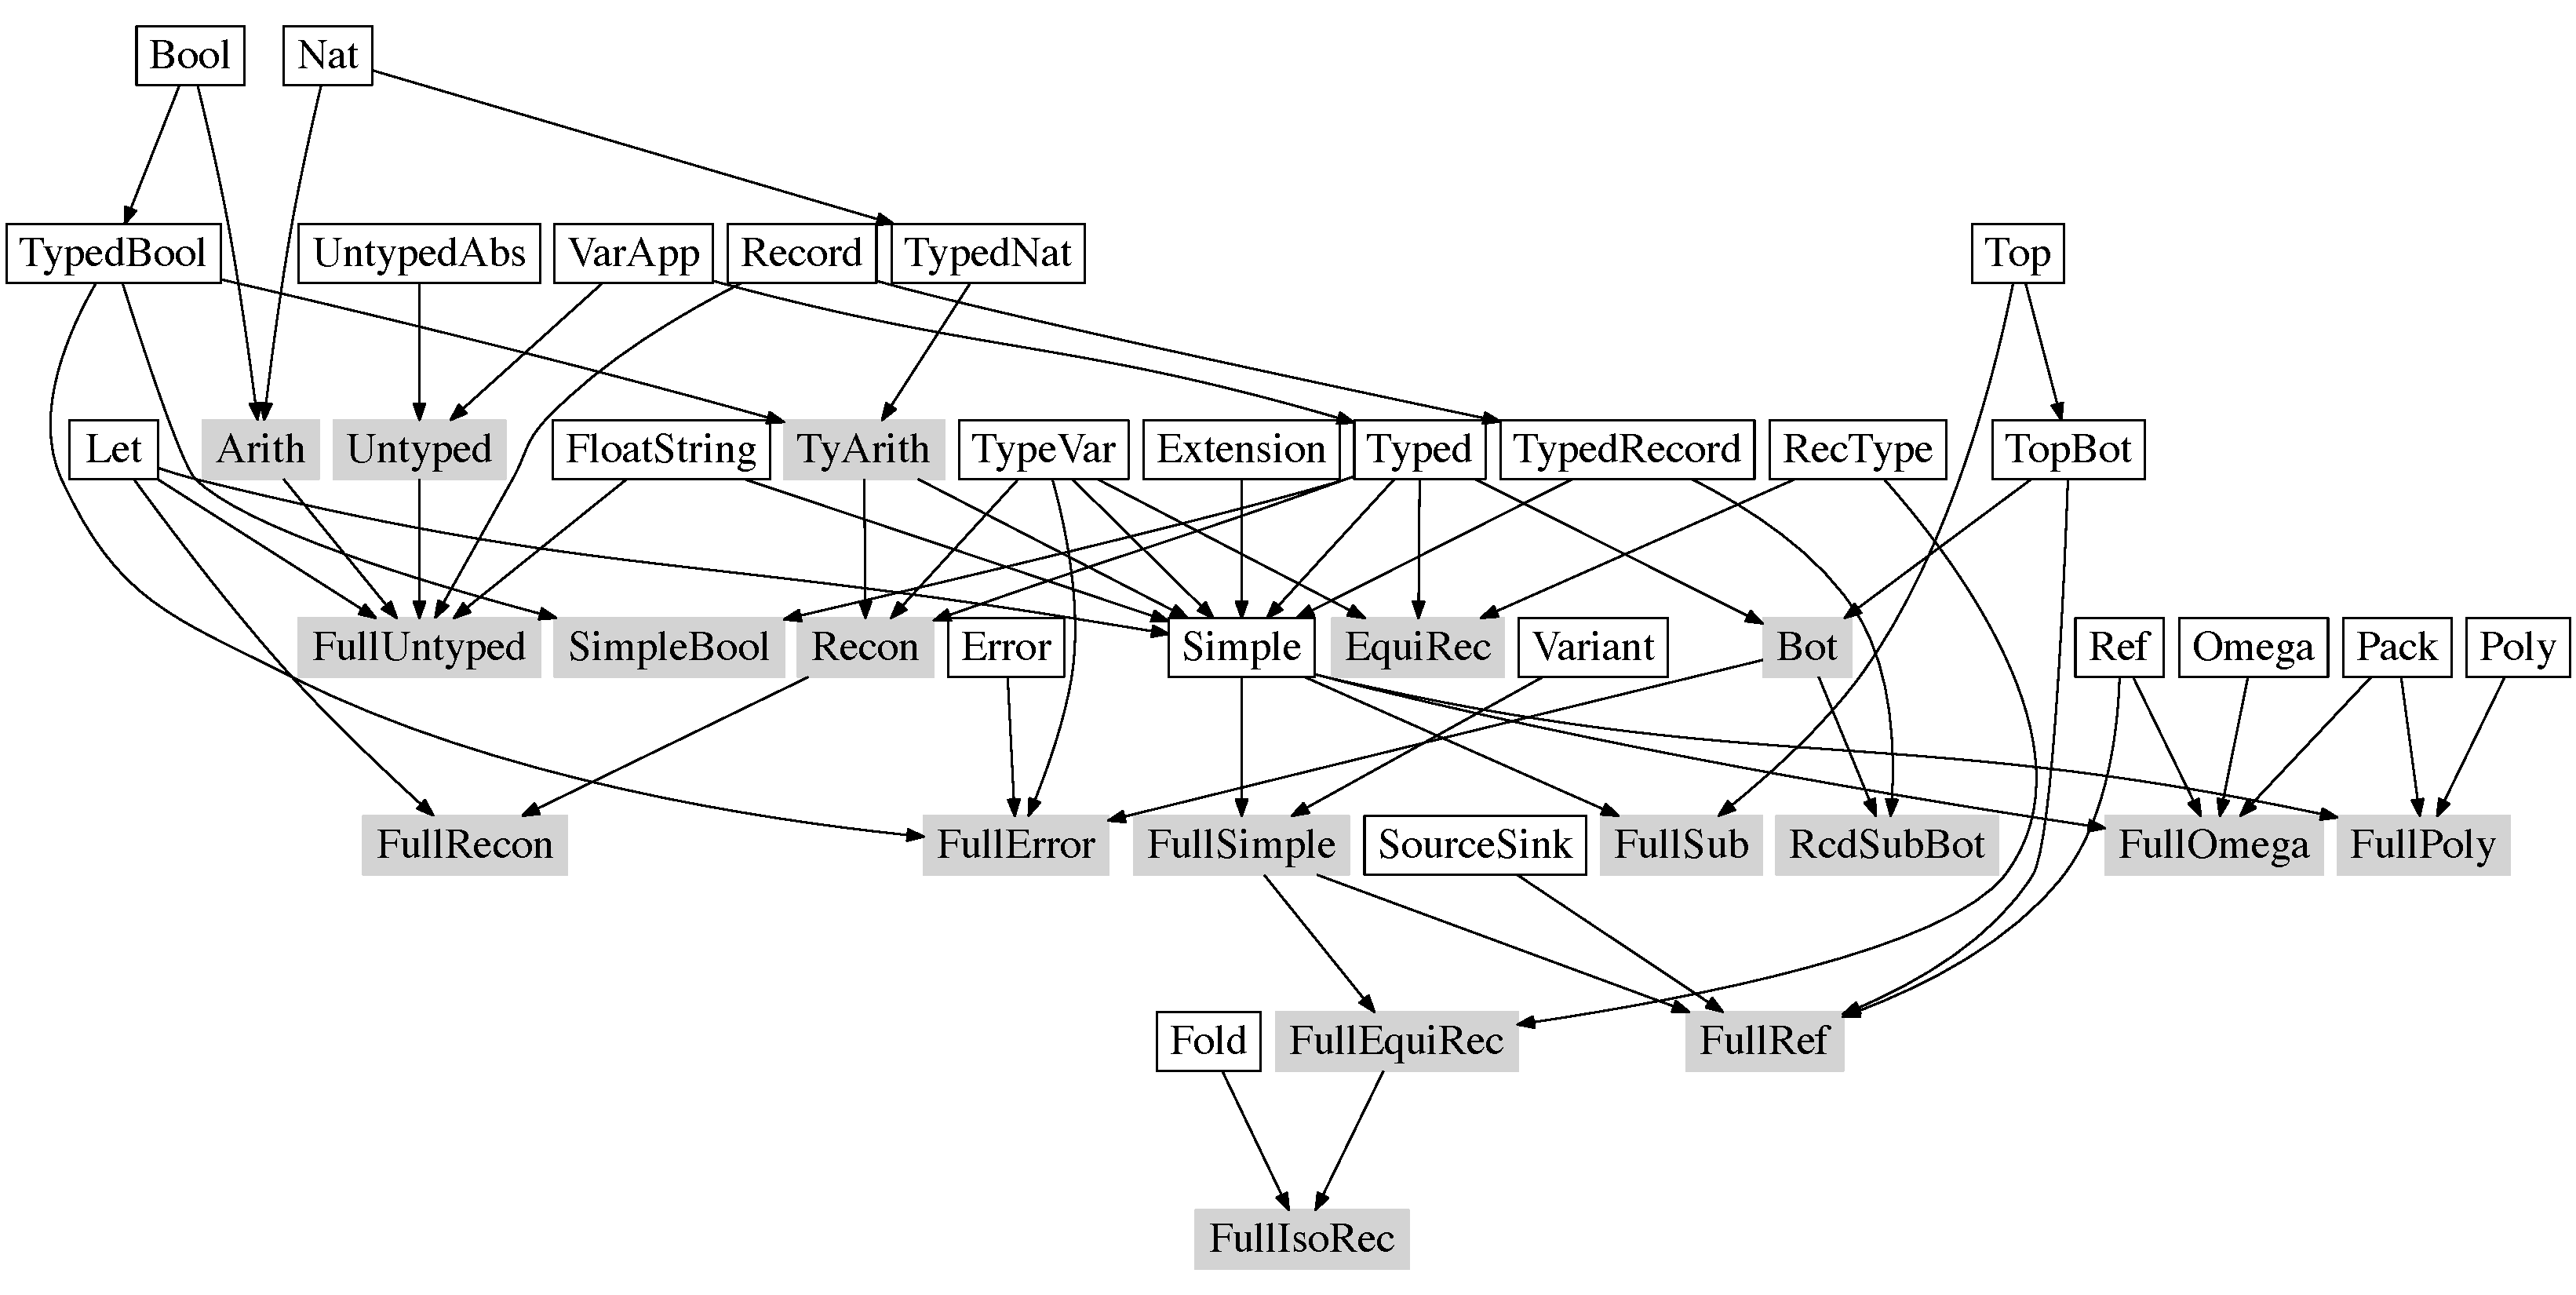
\includegraphics[width=0.8\textwidth]{resources/depGraph.pdf}
    \caption{Dependency graph of all calculi and components. Grey boxes are calculi; white boxes are components.}
    \label{fig:dependency}
\end{figure*}

Each component or language is represented by a Scala object which includes \lstinline{Alg}
for the abstract syntax, \lstinline{Print} for pretty-printing, and \lstinline{Parse} for parsing.
Since calculi and components have similar signatures, each calculus
can also be extended and reused directly. For example, calculus \lstinline{FullRef} extends from
calculus \lstinline{FullSimple}.

%% We have some naming conventions in our code, \lstinline{E} represents
%% expressions, \lstinline{T} represents types and \lstinline{K}
%% represents kinds. They are the three sorts of syntax in our case study.
%% In the component \lstinline{VarApp} we only have expressions. We use some helper traits for eliminating duplicate definitions, such as \inlinecode{EParser} containing \inlinecode{pE} for parsing expressions.

%% \lstinputlisting[linerange=9-9]{code/src/papercode/Sec6CaseStudy/Code1.scala}% APPLY:linerange=CASESTUDY_EPARSER

%% \paragraph{Composing Language Components}


%% The code of building \lstinline{Untyped} is presented in Figure~\ref{fig:casestudy-untyped}. Note that in the parser \inlinecode{Parse}, we need to override the object algebra interface and
%% parsing functions accordingly.

%% \begin{figure}[t]
%% \lstinputlisting[linerange=33-60]{code/src/papercode/Sec6CaseStudy/Code1.scala}% APPLY:linerange=CASESTUDY_UNTYPED
%% \caption{Build the \inlinecode{Untyped} calculus by composing to language components.}\label{fig:casestudy-untyped}
%% \end{figure}


%% \paragraph{Dependency Overview}

%% As shown in the graph, some components such as \lstinline{VarApp} are
%% created from scratch, while others such as \lstinline{Typed} are
%% extended from existing components.

%% From the graph, we know that common components such as \lstinline{VarApp} are reused in
%% lots of calculi. Such reuse could shorten the code considerably.
%% Next subsection examines amount of code as well as performance.

\vspace{-3pt}
\subsection{Comparison}\label{subsec:cs-comparison}

\newcommand\ourimpl{$\texttt{Mod}_{\texttt{OA}}$}
\newcommand\ilyaimpl{\texttt{NonMod}}
\newcommand\ourclass{$\texttt{Mod}_{\texttt{CLASS}}$}
\newcommand\ilyalongest{$\texttt{NonMod}_{\texttt{|||}}$}

We compared our implementation (named \ourimpl{}) with an implementation
available online\footnote{https://github.com/ilya-klyuchnikov/tapl-scala/} (named \ilyaimpl{}).
\ilyaimpl{} is suitable for comparison, because it is also
written in Scala using the same parser combinator library.
\ilyaimpl{} implements parsers 18 calculi in TAPL in a non-modular
way. Thus \ilyaimpl{} is not able to reuse existing
code when those calculi share common features.
\ourimpl{} implements the same 18 calculi, but reuse 
is possible due to modularity.

The comparison is made from two aspects. First, we want to discover
the amount of code reuse using our modular parsing approach.
For this purpose, we measured source lines of code (SLOC) of two implementations.
Second, we are interested to assess the performance penalty caused by modularity.
Thus we compared the execution time of parsing random expressions between two implementations.

\paragraph{Standard of Comparison}
In terms of SLOC, all blank lines and comments are excluded,
and we formatted the code of both implementations to ensure that
the length of each line does not exceed 120 characters. Furthermore,
because \ilyaimpl{} has extra code like semantics,
we removed all irrelevant code, only kept abstract
syntax definition, parser and pretty-printer for each calculus, to
ensure a fair comparison.

For the comparison of execution time, we built a generator to randomly
generate valid expressions for each calculus, according to its syntax. These expressions are
written to test files, one file per calculus. Each test file consists of 500
expressions randomly generated, and the size of test files varies from 20KB to 100KB.
We run the corresponding parser to parse the file and the pretty-printer to print the result.
The average execution time of 5 runs excluding reading input file was calculated, in milliseconds.

\begin{table*}\tiny
    \centering
    \resizebox{0.7\textheight}{!}{
    \begin{tabular}{|l|r|r|r|r|r|r|r|r|r|r|}
      \hline
        \multirow{2}{*}{\bfseries Calculus Name} & \multicolumn{3}{ c| }{\bfseries SLOC} & \multicolumn{7}{ c| }{\bfseries Time (ms)} \\ \cline{2-11}
        \multicolumn{1}{|c|}{} & \ilyaimpl{} & \ourimpl{} & \bfseries (+/-)\% & \ilyaimpl{} & \ourimpl{} & \bfseries (+/-)\% & \ilyalongest{} & \bfseries (+/-)\% & \ourclass{} & \bfseries (+/-)\% \\
      \hline
      \begin{tabular}{|c|c|c|}
  \hline
  t1 & t2 & t3 \\
  y1 & val1 & val4 \\
  y2 & val2 & val3 \\
  \hline
\end{tabular}

      \hline
      \multicolumn{7}{c}{}
    \end{tabular}}
 	\vspace{-5pt}
    \caption{Comparison of SLOC and execution time.}
    \label{tab:comparison}
    \vspace{-0.3cm}
\end{table*}

\vspace{-4pt}
\paragraph{Comparison Results}
Table \ref{tab:comparison} shows results of the comparison.
Let us only check \ourimpl{} and \ilyaimpl{} for now.
The overall result is that 69.2\% of code is reduced using our
approach, and our implementation is 42.7\% slower.

The good SLOC result is because of that the code of common language features
are reused many times in the whole case study. We can see that in the first two calculi
\lstinline{Arith} and \lstinline{Untyped} we are not better than \ilyaimpl{},
because in such two cases we do not reuse anything.
However in the following 16 calculi, we indeed reuse language components.
In particular, the calculi \inlinecode{EquiRec} and some others are only 22 lines
in our implementation, because we only compose existing code.

To discover the reasons of slower execution time, we made experiments
on two possible factors, which are Object Algebras and the longest match alternative combinator.
We use Object Algebras for ASTs and the longest match alternative combinator \inlinecode{|||} for parsing,
while \ilyaimpl{} uses case class and the ordinary alternative combinator.
Therefore, we implemented two more versions. One is a modified version of our implementation,
named \ourclass{}, with Object Algebras replaced by case class for the ASTs.
The other is a modified version of \ilyaimpl{}, named \ilyalongest{},
using the longest match alternative combinator instead of the ordinary one.

%% \begin{table*}
%%     \centering
%%     \begin{tabular}{|l|r|r|r|r|r|r|r|}
%%       \hline
%%         \multirow{2}{*}{\bfseries Calculus Name} & \ilyaimpl{} & \multicolumn{2}{ c| }{\ourimpl{}} & \multicolumn{2}{ c| }{\ilyalongest{}} & \multicolumn{2}{ c| }{\ourclass{}} \\ \cline{2-8}
%%         \multicolumn{1}{|c|}{} & \multicolumn{1}{c|}{\bfseries Time} & \bfseries Time & \bfseries (+/-)\% & \bfseries Time & \bfseries (+/-)\% & \bfseries Time & \bfseries (+/-)\% \\
%%       \hline
%%         Arith & 741 & 913 & +23.2 & 793 & +7.0 & 932 & +25.8 \\
%%         Untyped & 770 & 1018 & +32.2 & 821 & +6.6 & 1007 & +30.8 \\
%%         FullUntyped & 1297 & 1854 & +42.9 & 1343 & +3.5 & 1767 & +36.2 \\
%%         TyArith & 746 & 888 & +19.0 & 772 & +3.5 & 918 & +23.1 \\
%%         SimpleBool & 1376 & 1782 & +29.5 & 1494 & +8.6 & 1824 & +32.6 \\
%%         FullSimple & 1441 & 2270 & +57.5 & 1574 & +9.2 & 2226 & +54.5 \\
%%         Bot & 1080 & 1287 & +19.2 & 1078 & -0.2 & 1306 & +20.9 \\
%%       %\hline
%%         %\multicolumn{1}{|c|}{\dots} & \multicolumn{7}{c|}{\dots} \\
%%       %\hline
%%         FullRef & 1438 & 2291 & +59.3 & 1544 & +7.4 & 2142 & +49.0 \\
%%         FullError & 1410 & 1946 & +38.0 & 1524 & +8.1 & 1981 & +40.5 \\
%%         RcdSubBot & 1247 & 1524 & +22.2 & 1285 & +3.0 & 1612 & +29.3 \\
%%         FullSub & 1320 & 1979 & +49.9 & 1393 & +5.5 & 1899 & +43.9 \\
%%         FullEquiRec & 1407 & 2200 & +56.4 & 1561 & +10.9 & 2156 & +53.2 \\
%%         FullIsoRec & 1492 & 2253 & +51.0 & 1648 & +10.5 & 2236 & +49.9 \\
%%         EquiRec & 994 & 1254 & +26.2 & 1048 & +5.4 & 1304 & +31.2 \\
%%         Recon & 1044 & 1482 & +42.0 & 1128 & +8.0 & 1506 & +44.3 \\
%%         FullRecon & 1094 & 1645 & +50.4 & 1161 & +6.1 & 1652 & +51.0 \\
%%         FullPoly & 1398 & 2086 & +49.2 & 1511 & +8.1 & 2019 & +44.4 \\
%%         FullOmega & 1451 & 2352 & +62.1 & 1582 & +9.0 & 2308 & +59.1 \\
%%       \hline
%%         Total & 21746 & 31024 & +42.7 & 23260 & +7.0 & 30795 & +41.6 \\
%%       \hline
%%         \multicolumn{8}{c}{}
%%     \end{tabular}
%%     \caption{Execution time of four implementations.}
%%     \label{tab:ext-comparison}
%% \end{table*}

The right part of Table \ref{tab:comparison} suggests that the difference of running time between
using Object Algebras and class is little, roughly 1\%.
The use of longest match combinator slows the performance by 7\%. The main reason of slower
execution time may be the overall structure of the modular parsing approach, because we indeed have
more intermediate function calls and method overriding. However, it is worth mentioning that
because of the memoization technique of Packrat parsers, we are only constant times
slower, the algorithmic complexity is still the same.
Since the slowdown seems to be caused by extra method
dispatching, in future work we wish to investigate techniques like
partial evaluation or meta-programming to eliminate such cost. The
work by B{\'e}guet and Manohar~\cite{Beguet:2014} is an interesting starting point.


\section{Related Work}\label{sec:relatedwork}

%- extensible parsing, language workbenches: rats, noa (this one already uses OA), modular semantic actions, (syntactic modularity, no separate compilation, modular type-checking)
%(read more papers, see if they talk about this issue, some potential solutions)
%(attribute grammars?)
%
%- parser combinators for type-checking, previous work has not shown how to support modularity (ASTs); left-recursion and back-tracking in related techniques
%
%- modularity: object algebras, dtc and mrm (problem with parsing, is there any related work? (PB: a paper on unfolds: build the AST))
%
%(parsing in Javascript: using delegation, does it support modular AST)
%
%noa, shy: shy: only override some interesting cases (transformation is tedious)
%bruijn indices: parsing + transformation

Our work touches upon several topics including extensible parsing,
parser combinators and extensibility techniques. However, as far as we
know there's no work that discusses how to do statically type-safe and
separately compilable modular parsing.

\begin{comment}
There has been a
great amount of related papers on those topics. Some
inspired us of this paper and encourage us for more exploration. This
section will try to lead a discussion on what difference we have made.
\end{comment}

\paragraph{Syntactically Extensible Parsing}
Extensible parser generators~\cite{antlr1995,Grimm2006,Gouseti2014,Warth2016}
are a mainstream area of modular syntax and parsing. They allow users to write
modular grammars, where new
non-terminals and production rules can be introduced, some can even
override existing rules in the old grammar modules. For instance,
\textit{Rats!}~\cite{Grimm2006} constructs its own module system for
the collection of grammars, while NOA~\cite{Gouseti2014} uses Java
annotation to collect all information before producing an ANTLR~\cite{antlr1995} grammar
and the parsing code. Those parser
generators focus on the \textit{syntactic extensibility} of grammars:
they rely on whole compilation to generate a global parser, even if
there is only a slight modification in the grammar. Some of those
parser generators may statically check the correctness and unambiguity
of grammars. In contrast, because our approach is based on parser
combinators, there is no support for ambiguity checking.  However, as
far as we are aware, no extensible parser generators support separate
compilation or modular type-checking.

Macro systems like the C preprocessor, C++ templates and
Racket~\cite{Tobin-Hochstadt2011}, and other meta-programming
techniques are a similar area aiming at syntactic extensibility.
SugarJ~\cite{Erdweg2011} conveniently introduces syntactic sugar for
Java using library imports. Composition of syntactic sugar is easy for
users, but it requires many rounds of parsing and adaption, hence
significantly affects the efficiency of compilation. Since the
implementation was based on SDF~\cite{Heering1989} and
Stratego~\cite{Visser2001}, it does not support separate
compilation. Racket adopts a macro system for library-based language
extensibility~\cite{Tobin-Hochstadt2011}. It uses
attributed ASTs for contextual
information, and extensions can be integrated in a modular
way. However such modularity is not flexible enough for language
unification, as the syntax is only built from extensions.
%Moreover,
%existing macros cannot be further changed after
%definition. \haoyuan{correct?}
Extensible
compilers like JastAdd~\cite{Ekman2007} and
Polyglot~\cite{Nystrom2003} also support extensible parsing, but this
is mostly done using parser generators. They focus on the
extensions to a host language. Those techniques are short of type safety in a modular
setting as well.

%\bruno{Have you read
%Languages as Libraries? That is probably an important reference, which
%I think we should cite.}
%\haoyuan{what about
%  metafront? it is a macro system but does it have type safety?}
%\haoyuan{Extensible syntax with lexical scoping?} \haoyuan{"Extensible
%  syntax" proposes a system for extensible syntax, where users write
%  EDSLs in their language with concrete syntax. Users can write rules
%  for type-based disambiguation. But separate compilation is again not
%  mentioned. Shall we mention that thesis?} \haoyuan{attribute
%  grammars?}

\paragraph{Extensible Parsing Algorithm}
\textit{Parse table composition}~\cite{bravenboer2008parse}
is an approach where grammars are compiled to
modular parse tables. Those parse tables are expressed as DFAs
or NFAs, and later they can be composed by an algorithm, to provide
separate compilation for parsing. The generation of parse tables can
be quite expensive in terms of performance. The approach
is quite different from ours, since it uses parse
 tables, whereas we use parser combinators.
Our approach supports both
\emph{separate compilation} as well as \emph{modular
  type-checking}. Moreover, the extensibility of parsing is further
available at language composition and lexical level.

%\haoyuan{we do not have explicit
%  correspondence/relationship between abstract syntax and the parser.}

\paragraph{Parser Combinators} Parser combinators have become more and more
popular since~\cite{burge1975,Wadler1985}. Many parsing libraries produce recursive descent
parsers by introducing functional monadic
parser combinators~\cite{nott237}. Parsec~\cite{Leijen2001} is
perhaps the most popular parser combinator library in this line.
It is widely used in Haskell (with various ``clones'' in other languages)
for context-sensitive grammars with infinite lookahead. Nevertheless,
Parsec users suffer from manual left-recursion elimination,
high cost for backtracking and longest match composition issues,
as we discussed in Section~\ref{subsec:challenges}. Those limitations make Parsec
(and similar parsing techniques) inadequate for modular parsing.

Some more recent work on parser
combinators~\cite{Ford2002,Might2011,Frost2008} proposed a series of
novel parsing techniques that address the issue of
left-recursion. We have selected Packrat parsing due to its simplicity in Scala,
but in general it can also have alternatives.

\paragraph{Extensibility} Various design patterns~\cite{gamma1995design} in multiple
languages, have been proposed over the years to address extensibility
problems, such as the Expression Problem~\cite{wadler1998expression}.
The famous ``Datatypes \`a
la Carte'' (DTC)~\cite{swierstra2008data} approach represents modular ASTs using co-products
of every two functors. Several variants of DTC have been later proposed~\cite{Bahr2011,Bahr2014,Oliveira2015}.
All of that work essentially covers how to traverse and
consume extensible ASTs. However they do not
address the problem of \emph{modularly
parsing extensible ASTs}. Only in Bahr's~\cite{Bahr2011} work \emph{unfolds} is briefly mentioned,
yet it does not cover parsing.

There are also many design patterns in OO languages that achieve
type-safe extensibility~\cite{torgersen2004expression,odersky2005independently,oliveira2009modular,Oliveira:2012,wang2016expression}. We chose Object Algebras~\cite{Oliveira:2012} because the pattern is
relatively lightweight and makes good use of existing OO features,
such as inheritance, generics and subtyping. As seen throughout the paper,
the parsing code is concise and expressive using Object Algebras.
On the other hand we are unware of any work on OOP
that has covered how to do modular parsing for extensible ASTs.

It is worth mentioning that Scala case classes~\cite{emir2007matching} provide a near
solution to the Expression Problem. Case classes can be
modularly added, but they do not enforce
exhaustiveness of pattern matching for extensible operations. In other
words run-time pattern matching errors can happen when writing extensible code with case classes. So that full static type-safety is not ensured. Nevertheless case classes are a pragmatic approach, which is
widely used in practice. Therefore, modular parsing techniques may be
of value for extensible code using case classes.  The approach we
presented in Section~\ref{sec:inheritance} can readily be adapted to case classes:
all that the users need to do is to use case classes, instead of
standard OO classes in their code.

\begin{comment}
Moreover, in~\cite{Oliveira:2012} the authors have discussed the
composition of algebras. In our parsing approach, a parser consumes an
algebra, which is delegated to return the results, during its process
of parsing. Having a set of algebras, it requires multiple parsing
with several times of invocation, which leads to redundant work.
Instead, algebras are supposed to be composed into one before the
invocation of the parser. Bahr et al. lead a similar discussion
in~\cite{Bahr2011}, where queries (or \textit{catamorphisms}) and
transformations (or \textit{homomorphisms}) are composable. They have
also mentioned the dual process of folds, namely
\textit{anamorphisms}. It is potentially related to our work, as
parsing is a representative kind of unfolds, whereas they only
discussed the composition of a cv-coalgebra and a term homomorphism,
which differs from modular parsing.
\end{comment}

\begin{comment}
Another interesting observation from Section~\ref{sec:algebrasandparsing}, is that parsers with
Object Algebras generate ``implicit objects'', which are actually functions of
type \lstinline{Alg[E]} \lstinline{=>} \lstinline{E} for generic \lstinline{E}.
Patterns of operations on such functions are captured by the original paper~\cite{Oliveira:2012}, called
\textit{queries} and \textit{transformations}, together with the composition of algebras.
They are quite useful, for instance, we have two operations (like the aforementioned \lstinline{Print} and \lstinline{Eval}) to be fed to the parser. If we feed them separately, it is tedious to parse the same input twice. Instead we can compose them in advance before the feeding. On the other hand, one would think this pattern is too limited to use against objects that traditional parsers generate. For example, there are a lot of transformations (or desugarings) on intermediate ASTs in the design of a compiler. Transformation algebras are helpful in that case. They can even be composed in a linear pipeline-style before a query algebra is delegated. The Shy framework~\cite{Zhang2015} has captured those patterns, and it generates templates for them, so that users only need to override a few interesting cases, conveniently. The idea of overriding existing cases was also
proposed in MRM~\cite{Oliveira2015}. They are potentially useful to our approach. Regarding overriding, our approach allows existing parsing code to be overridden during inheritance.
\end{comment}


\section{Conclusion}\label{sec:conclusion}

This paper presents a solution for semantically modular parsing. It not only
enables parsers to evolve with the syntax together, but also allows them to be modularly type-checked and separately compiled.

Based on parser combinators, we identify the the algorithmic challenges of building modular parsers, and show that Packrat parsing is suitable as the underlying parsing technique. Our solution does not require advanced language features. We show that with standard OO techniques including inheritance and overriding, it is practicable to build modular parsers for OO ASTs. However, the extensibility issue of traditional OO ASTs motivates us to adopt Object Algebras for full extensibility and more useful features.

Abstracting language features as reuseable components can be achieved based on our solution, which is useful for rapid language prototyping. Our solution does not rely on particular techniques. On the contrary, it is a general framework customizable by the user. The TAPL case study shows that we can obtain considerable code reuse (69\%) than a non-modular implementation, using our modular parsing approach and language feature abstraction.

There are certainly some aspects can be improved. We observed that the glue code of composition appears to be boilerplate. Such an issue refers to family polymorphism, and we could solve it by language features or meta-programming techniques. Moreover, we can possibly adopt the Shy framework~\cite{Zhang2015} and algebra composition patterns~\cite{oliveira2013feature}, to improve the usage of Object Algebras.

For future work, we will experiment more on how open recursion contributes to extensible parsing in functional languages, by making use of laziness. It is also interesting to see that parsing, to some extent, can be viewed as a special example of \textit{unfolds}. So it is worthwhile considering to generalize our approach under certain circumstances.


%===============================================================================

\bibliographystyle{plain}
\bibliography{paper}

\appendix

\end{document}

%%% Local Variables:
%%% mode: latex
%%% TeX-master: "."
%%% End:
